\chapter{Modello Lineare Classico} 
Un generico modello di regressione esprime una relazione del tipo:
\begin{equation}
	y = f(x_1, \dots, x_k) + \varepsilon
\end{equation}
dove la $y$ è la variabile dipendente che si cerca di spiegare in termini delle variabili indipendenti $x_1, \dots, x_k$ dette anche variabili \textit{esplicative}, \textit{regressori} o \textit{covariate}.$\varepsilon$ rappresenta invece la componente di errore circa la relazione che lega la $y$ alle covariate $x$, che può essere dovuta ad errori individuali, errori di misurazione o omissione di variabili esplicative che potrebbero ulteriormente cogliere la relazione che sussiste tra $y$ e $x$.

Esistono diversi modelli di regressione, in questa dispensa in particolare viene indagato il metodo di regressione lineare che può essere:
\begin{itemize}
	\item \textbf{semplice}, se si utilizza una sola variabile esplicativa, quindi:
	\begin{equation}
		y_i = \beta_0 + \beta_1 x_1 + \varepsilon
	\end{equation}
	dove si è utilizzato il pedice $i$ per la $y$ per specificare la specifica relazione tra l'osservazione $i$ del campione o della popolazione che si sta studiando e la variabile $x_1$ che in questo caso rappresenta il valore specifico che la covariata $x_1$ assume per l'osservazione $i$. 
	\item \textbf{multiplo}, se si inserisce più di una variabile esplicativa, quindi:
	\begin{equation}
		y_i = \beta_0 + \beta_1 \cdot x_1 + \beta_2 \cdot x_2 + \dots + \beta_k \cdot x_k + \varepsilon
	\end{equation}
	\item \textbf{multivariato}, se si ha più di una variabile dipendente e più di una variabile esplicativa, quindi:
	\begin{equation}
		\mathbf{y_1}, \mathbf{y_2}, \dots, \mathbf{y_n} = \beta_0 + \beta_1 \cdot x_1 + \beta_2 \cdot x_2 + \dots + \beta_k \cdot x_k + \varepsilon
	\end{equation}
\end{itemize}
Senza considerare per ora il caso multivariato che sarà analizzato in un prossimo capitolo, il modo più generale per esprimere la relazione tra una variabile dipendente e le variabili di regressione è la seguente:

\begin{equation}
Y = X \cdot \underline{\beta} + \underline{\varepsilon}
\end{equation}
dove con $Y$ si è indicato il vettore per tutte le osservazioni $i$ in studio, e con $X$ la matrice che contiene i valori delle covariate per ogni osservazione $i$ del modello (più il termine noto).
\begin{equation}
Y = 
\begin{pmatrix}
y_1 \\ 
. \\ 
. \\ 
. \\ 
y_n
\end{pmatrix}
\quad
X = \begin{pmatrix}
1 & x_{1,2} & \dots & x_{1,k} \\ 
1 & x_{2,2} & \dots & \vdots \\ 
\vdots & \dots  & \ddots & \vdots \\ 
1 & \dots &  & x_{n,k}
\end{pmatrix} 
\quad
\underline{\beta} = \begin{pmatrix}
b_0 \\ 
. \\ 
. \\ 
. \\ 
b_n
\end{pmatrix} 
\quad
\underline{\varepsilon} = \begin{pmatrix}
\varepsilon_0 \\ 
. \\ 
. \\ 
. \\ 
\varepsilon_n
\end{pmatrix} 
\end{equation}
La matrice $X$, detta anche \textit{matrice disegno}, ha la prima colonna composta da tutti $1$ in quanto questa colonna è quella che va a moltiplicarsi con il termine noto, che è il primo valore nel successivo vettore $\underline{\beta}$. Ogni colonna della matrice rappresenta una variabile esplicativa quindi la prima colonna per esempio rappresenta la variabile esplicativa $x_1$ e ogni elemento in questa colonna è il valreo che tale variabile assume per l'osservazione $i$, così che se si considera per esempio la prima osservazione il valore di $y$ per questa osservazione sarebbe la prima riga della moltiplicazione tra matrici a destra dell'equazione, ovvero:
\begin{equation}
	y_1 = \beta_0 + \beta_1 \cdot x_{11} + \dots + \beta_n \cdot x_{1n} + \varepsilon_1
\end{equation}
$\underline{\beta}$ rappresenta come si è detto il vettore dei parametri ignoti per i regressori, mentre $\underline{\varepsilon}$ quello degli errori per ciascuna osservazione.

\section{Ipotesi sul modello}
Il modello di regressione lineare fin qui presentato poggia la sua validità su una serie di ipotesi che sono qui riassunte.
\subsection{Ipotesi di Linearità}
Secondo questa ipotesi, sia le variabili esplicative del modello (i valori della matrice $\doubleunderline{X}$) sia i parametri $\underline{b}$ sono lineari.

\subsection{Ipotesi di Non Sistematicità degli Errori}
Quest'ipotesi sostiene che il valore atteso di ogni errore $\varepsilon_i$ dato il corrispondente set di variabili esplicative corrispondente alla riga $i$-esima della matrice $X$ è zero, ovvero:
\begin{equation}
E\left(\varepsilon_i|{X}_{in}\right) = 0
\end{equation}
Di conseguenza il valore atteso della variabile dipendente è:
\begin{equation}
E\left(\underline{y}|{X}\right) = X \underline{\beta}
\end{equation}

\subsection{Ipotesi di Sfericità degli Errori}
Per quest'ipotesi valgono le seguenti:
\begin{enumerate}
	\item Ipotesi di \textbf{omoschedasticità}, ovvero la  variabilità  dell'effetto  di  tutti  i  fattori  non  rilevati  e/o  non  rilevabili  non  dipende  dai 
	valori dei regressori. Quindi:
	\begin{equation}
	V(e \vert x_1, \dots, x_n) = \sigma^2 \quad \Rightarrow V(Y \vert x_1, \dots, x_n) = \sigma^2
	\end{equation}
	\item Ipotesi di \textbf{incorrelazione}, ovvero gli  effetti su y dei  fattori  non  rilevati $\varepsilon$  per  l'osservazione i non  dipendono  da  quelli relativi all'osservazione j. Quindi:
	\begin{equation}
	Cov(\varepsilon_i, \varepsilon_j) = 0 \quad \forall i, j
	\end{equation}
	dove $\varepsilon_i$ e $\varepsilon_j$ sono appunto il valore delle variabili aleatorie per le osservazioni $i$ e $j$.
	\item Gli errori devono essere distribuiti in modo normale con media zero e varianza $\sigma^2$:
	\begin{equation}
	\varepsilon \sim N(0,\sigma^2)
	\end{equation}
\end{enumerate}

A questo punto se abbiamo tante osservazioni la situazione diventa la seguente:

Le condizioni ipotizzate prima sulle singole osservazioni del modello continuano a valere e possono essere riscritte in maniera più compatta come segue:
\begin{enumerate}
	\item E($\underline{\varepsilon}$) = 0
	\item V($\underline{\varepsilon}$) = E($\underline{\varepsilon}$, $\underline{\varepsilon'}$) = $\doubleunderline{\Sigma}$ = $\sigma^2 \mathds{1}_n$ 
\end{enumerate}


\subsection{Ipotesi di Non Stocasticità delle Variabili Esplicative}
Si suppone che i valori delle variabili esplicative $\underline{x}_j$ siano fissi e non soggetti a fluttuazioni stocastiche. Di conseguenza vale:
\begin{equation}
E(\doubleunderline{X}) = \doubleunderline{X}
\end{equation}
Ossia il valore di aspettazione della matrice delle covariate è la matrice stessa. Inoltre la correlazione tra questa e il vettore degli errori è nulla, cioè:
\begin{equation}
cov(\doubleunderline{X},\underline{\varepsilon}) = 0
\end{equation}

\subsection{Ipotesi di Non Collinearità delle Variabili Esplicative}
I vettori delle variabili esplicative contenuti nella matrice $\doubleunderline{X}$ sono linearmente indipendenti. La matrice $\doubleunderline{X}$ ha rango pieno, pari al numero delle covariate più uno dovuto al vettore costante, cioè:
\begin{equation}
Rank(\doubleunderline{X}) = p + 1
\end{equation}
Di conseguenza, la matrice ha determinante non nullo, è invertibile e il prodotto $\doubleunderline{X}\cdot\doubleunderline{X}^T$ è definito.

\subsection{Ipotesi sulla Numerosità della popolazione}
Si suppone che il numero di eventi nel campione sia maggiore della numero di covariate (più uno a causa del vettore costante):
\begin{equation}
n > p + 1
\end{equation}
Questo garantisce che la matrice $\doubleunderline{X} \cdot \doubleunderline{X}^T$ abbia un'unica inversa, dunque la soluzione al problema di regressione sia unica.


\section{Estimatori}

Un'estimatore è una funzione da applicare su un certo campione di dati preso in maniera casuale dalla popolazione. La stima è il valore numerico che l'estimatore assume quando viene calcolato sul set. Ogni estimatore può essere classificato sulla base di tre criteri.

\subsection{Correttezza (Unbiasedness)}
Lo stimatore può essere applicato su diversi campioni casuali. Perchè sia un buon estimatore, ci si aspetta che la distribuzione dei suoi valori sia centrata sulla stima esatta che avrebbe sulla popolazione, cioè:
\begin{equation}
E(\hat{\mu}_Y) = \mu_Y
\end{equation}

dove $Y$ è la popolazione considerata, $\hat{\mu}_Y$ è l'estimatore applicato su un campione e $\mu_Y$ è l'estimatore applicato alla popolazione. Se un'estimatore possiede questa proprietà è detto corretto o unbiased, altrimento è detto scorretto o biased.

\subsection{Consistenza (Consistency)}
Un' estimatore è detto consistente se all'aumentare della dimensione del campione su cui viene applicato, questo tende ad assumere il valore vero. Ciò si può scrivere come:
\begin{equation}
\hat{\mu}_Y \xrightarrow{p} \mu_Y
\end{equation}

\subsection{Efficienza (Efficiency)}
Siano $\tilde{\mu}_Y$ e $\hat{\mu}_Y$ due estimatori della stessa quantità $\mu_Y$, entrambi corretti. Il criterio dell'efficienza dice che per scegliere quale estimatore tra i due sia migliore, si guarda alla larghezza della loro distribuzione (cioè alla loro varianza): l'estimatore con varianza minore è quello più efficiente, cioè:
\begin{equation}
var(\hat{\mu}_Y) < var(\tilde{\mu}_Y)
\end{equation}
\section{Il metodo dei minimi quadrati ordinari (OLS)}


Come metodo di stima dei parametri $b$ si può utilizzare il \textit{metodo dei minimi quadrati}.

Nell'ipotesi di perfetta dipendenza lineare tra $Y$e gli $n$ regressori è possibile, facendo un campione di osservazioni, stimare i valori \underline{teorici} previsti per la variabile dipendente $y$ per tutte le unità del campione. Facendo la differenza tra questi valori teorici previsti e quelli empirici che risultano dall'osservazione si definiscono i residui come:
\begin{equation}
\underline{e} = \underline{y} - \underline{y'} = \underline{y} - \doubleunderline{X} \cdot \underline{b}
\label{eq: residui}
\end{equation}
dove con $\underline{y'}$ si è appunto indicato il vettore dei valori teorici previsti facendo una stima di $b$ sul campione.
\begin{equation}
y'_i = b_0 + b_1 x_{1i} + b_2 \dots + b_n x_{ni} \quad \text{per} \; i= 1, \dots, k
\end{equation}
Quindi il singolo residuo nella \eqref{eq: residui} si può anche riscrivere come:
\begin{equation}
e_i = y_i - y'_i = y_i - b_0 + b_1 x_{1i} + b_2 x_{2i} + \dots + b_n x_{ni} \quad \text{per} \; i= 1, \dots, k
\end{equation}
I valori di $e_i$ sono $k$ determinazioni campionarie (per i $k$ campioni presi) del termine d'errore $\varepsilon$ del modello.\\
\textit{Oss.} È necessario fare campioni anche nel caso in cui abbiamo
molti dati, in quanto se ho molti dati la regione di accettazione
diventa piccolissima.
Il metodo dei minimi quadrati ricerca il vettore di coefficienti $\underline{b}$ in modo da rendere minima la somma dei quadrati degli scarti tra ordinate empiriche e ordinate teoriche, o equivalentemente, la somma dei residui al quadrato:
\begin{equation}
\Phi(\underline{b}) = \sum_{i=1}^k (y_i - y'_i)^2 = \sum_{i=1}^k e_i^2 = \underline{e}^t 	\cdot \underline{e} = (\underline{y} - \doubleunderline{X} \cdot \underline{b})^t \cdot (\underline{y} - \doubleunderline{X} \cdot \underline{b})
\end{equation}
Sviluppando il calcolo si minimizza la funzione ponendo = 0 la derivata rispetto a $b$, ovvero:
\begin{equation}
\frac{\partial \Phi(\underline{b})}{\partial \underline{b}} = 0
\end{equation}
che porta alla seguente equazione, detta \textit{equazione normale}:
\begin{equation}
\doubleunderline{X}^t \doubleunderline{X} \cdot \underline{b} = \doubleunderline{X}^t \underline{y}
\end{equation}
che corrisponde ad un sistema di $n+1$ equazioni in $n+1$ incognite. Nel caso in cui $k = 1$ si ha il modello di regressione lineare semplice. L'espressione tramite cui è stimato $\underline{b}$:
\begin{equation}
\underline{b} = (\doubleunderline{X}^t X)^{-1} \doubleunderline{X} \cdot \underline{y}
\end{equation}
prende il nome di \textit{stimatore dei minimi quadrati}.\\
Se le variabili sono standardizzate, ovvero divisi per lo scarto quadratico medio, lo stimatore dei minimi quadrati diventa:
\begin{equation}
\underline{b} = (\doubleunderline{X}^{*t} \doubleunderline{X}^*)^{-1} \doubleunderline{X}^{*t} \cdot \underline{y}^*
\end{equation}
dove $\doubleunderline{X}^* = \doubleunderline{X} \cdot \doubleunderline{D_x}^{-1/2}$ con $\doubleunderline{D_x}$ matrice i cui elementi diagonali sono le varianze delle variabili $x$ (ottenendo in questo modo le $x$ originali divise per il loro scarto quadratico medio), mentre $y^*$ è $y/\sigma_y$.

Il problema si può anche vedere dal punto di vista geometrico. Possiamo infatti identificare il sottospazio lineare di $\mathbb{R}^N$ delle colonne di $\doubleunderline{X}$, e in questo spazio la somma:
\begin{equation}
\sum_{i=1}^k (y_i - y'_i)^2 = \sum_{i=1}^k (y_i - \doubleunderline{X} \cdot \underline{b})^2
\end{equation}
è il quadrato della distanza euclidea tra $\underline{y}$ e $\doubleunderline{X} \cdot \underline{b}$., ovvero:
\begin{equation}
\sum_{i=1}^k (y_i - \doubleunderline{X} \cdot \underline{b})^2 = \| y_i - \doubleunderline{X} \cdot \underline{b} \|^2
\end{equation}
Chiamiamo $\mu = \doubleunderline{X} \cdot b$ il nostro vettore dei valori fittati (i valori teorici previsti) che corrisponde ad un vettore nello spazio delle colonne di $\doubleunderline{X}$ . Questo vettore $\mu$ rappresenta anche l'unica proiezione di $\underline{y}$ su $\doubleunderline{X}$. La distanza tra $\underline{y}$ e $\mu$ è un vettore ortogonale (vettore dei residui) allo spazio $\doubleunderline{X}$ e il metodo dei minimi quadrati ha lo scopo di minimizzare questo vettore. Se la dimensione dello spazio delle colonne è esattamente uguale al numero di variabili esplicative allora la soluzione è unica.
%\begin{figure}
%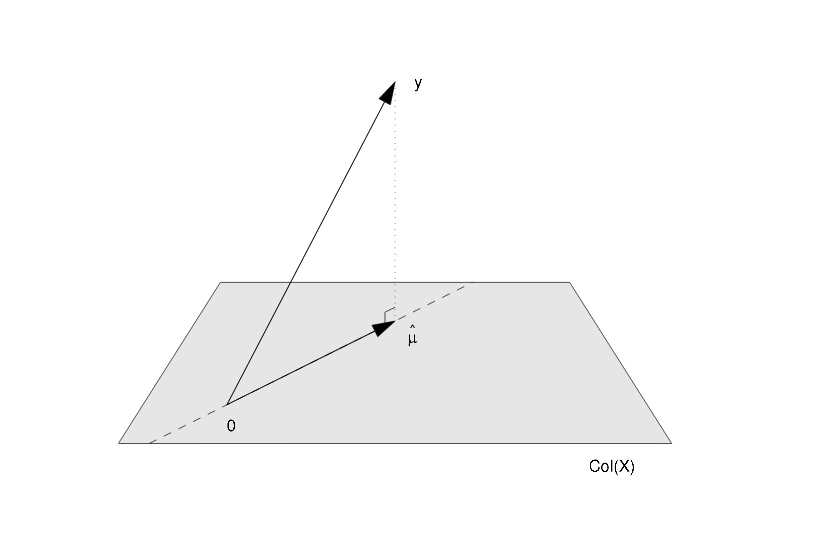
\includegraphics[scale=0.4]{Immagini/spazio-col.png}
%\caption{Rappresentazione dello spazio delle colonne e dei vettori di interesse.}
%\end{figure}
\section{Bontà di adattamento}
La bontà di adattamento si stima in base a \textit{devianza totale} e
\textit{devianza spiegata}.\\
La \textit{devianza spiegata} è la somma delle differenze al quadrato tra i valori teorici della retta interpolante e la media dei valori empirici.\\
La \textit{devianza residua} è la somma degli scarti al quadrato tra i valori osservati e teorici della $y$. \\
La \textit{devianza totale} è la somma degli scarti dei valori di $y$ empirici dalla loro media.

L'indice di adattamento è definito come:
\begin{equation}
R^2 = \frac{DevSpieg(Y)}{DevTot(Y)}
\end{equation}
Nel caso di un modello di regressione lineare semplice si ha che:
\begin{equation}
DevSpieg(Y) = b_1 Codev(X, Y)
\end{equation}
Dividendo per $n-1$ e con opportuni passaggi (si veda http://www2.stat.unibo.it/montanari/Didattica/lab3.pdf) si arriva a:
\begin{equation}
R^2 = \frac{Cov(X, Y)}{var(X)var(Y)}
\end{equation}

$R^2$ è un numero che varia tra 0 e 1, è = 0 se non c'è correlazione lineare, = 1 se c'è perfetta correlazione.

\section{Testare i risultati: t-test e F-measure (test di ipotesi)}
Per testare i risultati ottenuti dei parametri si possono effettuare due misure di test sull'ipotesi nulla che il coefficiente stimato sia o meno uguale a zero, ovvero:
\begin{equation}
H_0 = \beta_i = 0
\end{equation}

\subsection{Test di ipotesi e \textit{p-value}}
Un test di ipotesi è un procedimento tramite il quale si verifica la validità di una certa ipotesi. Solitamente si parte definendo un'\textit{ipotesi nulla} tramite la quale si afferma che per la popolazione, o comunque più in generale per il fenomeno che si sta studiando, vale una determinata condizione, ovvero:
\begin{equation}
H_0 = \mu 
\end{equation}
dove $\mu$ sta a indicare una qualsiasi condizione che si vuole testare. \\
L'\textit{ipotesi alternativa} invece specifica che cosa è vero nel caso in cui l'ipotesi nulla sia falsa. La più generale ipotesi alternativa è il contrario dell'ipotesi nulla ovvero:
\begin{equation}
H_1 \neq \mu 
\end{equation}
La valutazione dei risultati di un test di ipotesi avviene considerando il cosiddetto \textit{p-value}. Per calcolare il p-value si calcola prima la distribuzione di probabilità per l'ipotesi nulla, assumendo quindi che essa sia vera si costruisce la distribuzione di probabilità centrata su questo valore, ed in seguito bisogna calcolare la probabilità di ottenere un valore che sia più grande del valore medio osservato per la quantità che si sta studiando. La distribuzione di probabilità che si costruisce infatti è una distribuzione delle  medie, e il valore osservato è una media ottenuta da un campione.\\ 
Il p-value è quindi l'area sottesa alla parte di curva a destra del valore osservato.
Vogliamo che la probabilità evidenziata sia la più piccola possibile, ovvero che il valore osservato sia il più possibile discostato dal centro della curva in quanto essa è centrata sull'ipotesi nulla. Se stabiliamo un livello di confidenza $\alpha$ ciò significa che la \textit{probabilità} di ottenere un valore uguale o più grande del valore osservato deve essere minore o uguale a $\alpha$. Quindi la parte di curva (probabilità) dentro le regioni delle code esterne individuate da $\alpha$ è uguale a $1-\alpha$.
\begin{equation}
P(-Z_{\frac{\alpha}{2}}< \bar{a} < +Z_{\frac{\alpha}{2}}) = 1 - \alpha
\end{equation}
Dove $-Z_{\frac{\alpha}{2}}$ e $+Z_{\frac{\alpha}{2}}$ rappresentano i valori di $\bar{a}$ tali per cui la probabilità racchiusa all'interno di questi valori è uguale a $1-\alpha$. 
\begin{figure}
	\centering
	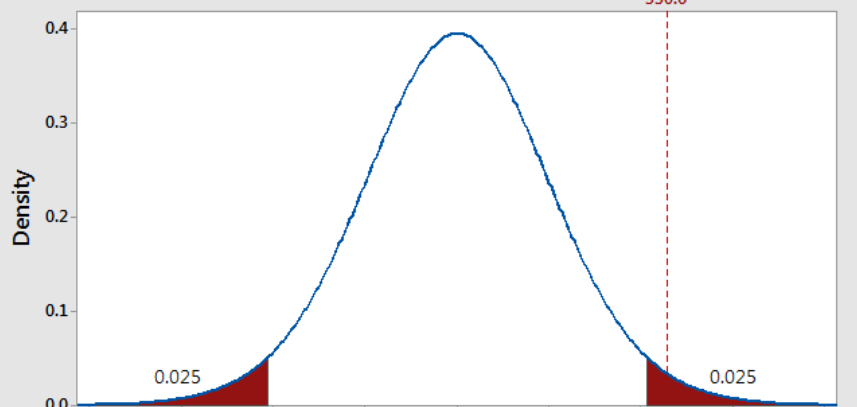
\includegraphics[scale= 0.3]{Immagini/distro-pvalue.png}
	\caption{La curva rappresenta la distribuzione centrata sull'ipotesi nulla, le parti colorate di rosso rappresenta invece il livello $\alpha$ in questo caso uguale al $5\%$, quindi, essendo la curva simmetrica sarà $0,025$ a destra, e $0,025$ a sinistra. La linea tratteggiata rappresenta invece il valore osservato che in questo caso cade all'interno dell'area accettata per rifiutare l'ipotesi nulla.
		credits: http://blog.minitab.com/blog/adventures-in-statistics-2/understanding-hypothesis-tests:-significance-levels-alpha-and-p-values-in-statistics}
	\label{fig: distro-pvalue}
\end{figure}
Se standardizziamo la distribuzione della quantità $\bar{a}$ in modo da renderla a media nulla e varianza 1 (quindi sottraiamo la media e dividiamo per la deviazione standard), otteniamo:
\begin{equation}
P\left(-Z'_{\frac{\alpha}{2}}< \frac{\bar{a} - \mu_a(H_0)}{\sigma} < +Z'_{\frac{\alpha}{2}}\right) = 1 - \alpha
\end{equation}
che implica che $\bar{a}$ deve trovarsi entro i seguenti valori in termini di deviazione standard rispetto alla media:
\begin{equation}
\label{eq: prob-interna}
P\left(\mu_a(H_0) - Z'_{\frac{\alpha}{2}} \cdot \sigma < \bar{a} < \mu_a(H_0) + Z'_{\frac{\alpha}{2}} \cdot \sigma \right) = 1 - \alpha
\end{equation}
I valori di $Z'$ sono tabulati dalla funzione degli errori.\\
La probabilità (p-value) per un valore osservato di $\bar{a}$ è:
\begin{equation}
p = P\left( \left| \frac{\bar{a} - \mu_a(H_0)}{\sigma} \right| > \left| \frac{\bar{a_{oss}} - \mu_a(H_0)}{\sigma} \right| \right)
\end{equation}
che rappresenta quindi la probabilità di osservare un valore di $\bar{a}$ maggiore o uguale a quello che si è osservato (supponendo valida l'ipotesi nulla). Se questo valore di probabilità è inferiore al livello $\alpha$ fissato (quindi il valore $\bar{a_{oss}}$ è al di fuori dell'intervallo individuato in termini di $Z'$ intervalli di confidenza) si può rigettare l'ipotesi nulla.

\begin{tcolorbox}[colback=cyan!5!white, colframe=cyan!75!black, title = Il livello di confidenza $\alpha$]
	A livello interpretativo il livello di confidenza $\alpha$ che si specifica (solitamente è fissato a $0,05$, ovvero al $5\%$ totale della distribuzione) indica la probabilità di rigettare l'ipotesi nulla nel caso in cui poi essa sia effettivamente vera, ovvero le probabilità di errore. Nel valutare l'ipotesi nulla infatti possiamo incappare in due tipi di errori: ritenerla vera quando invece in realtà è falsa, e ritenerla falsa quando invece in realtà è vera. Specificando il livello $\alpha$ stiamo specificando la probabilità di commettere il secondo tipo di errore, infatti se diciamo che rifiutiamo l'ipotesi nulla se il valore che osserviamo cade nelle code, ovvero nella regione $\alpha$ della curva, stiamo comunque rifiutando tutti quei valori della distribuzione per cui l'ipotesi nulla è comunque vera, anche se poco probabile. Quindi nel caso in cui poi l'ipotesi nulla sia effettivamente vera, al massimo in $\alpha \; ( e.g.\!5\%)$ dei casi concluderemo che è falsa, in quanto troveremo i valori nelle code per cui abbiamo deciso si rifiutare l'ipotesi, mentre nel rimanente $95\%$ concluderemo correttamente che è vera. Se invece è effettivamente falsa queste probabilità non valgono più.
\end{tcolorbox}

\subsection{t-test}

La \textit{t-statistic}, detta anche \textit{t-measure} o \textit{t-test}, rappresenta un modo per valutare se la stima di una quantità risulta accettabile o meno rispetto ad un'ipotesi nulla. È definita come segue:
\begin{equation}
t = \frac{a - a_0}{SE(a)}
\end{equation}
dove $a_0$ è il valore dell'ipotesi nulla che si sta testando per la quantità $a$ e $SE$  è lo \textit{standard error} di questa variabile ovvero: $\frac{\sigma}{\sqrt{n}}$.\\
Quindi nel caso della stima dei parametri $\beta$ della regressione lineare semplice, in cui per l'ipotesi nulla si suppone che $\beta$ abbia valore zero,  si ha:
\begin{equation}
t = \frac{\beta_i}{SE(\beta_i)} = \frac{\beta_i}{\frac{\sigma}{\sqrt{n \sigma_{jj}}}}
\end{equation}
se la $\sigma$ è nota, altrimenti si usa il suo stimatore $s$, quindi:
\begin{equation}
t = \frac{\beta_i}{\frac{s}{\sqrt{n \sigma_{jj}}}}
\end{equation}
Se si fissa quindi un livello di confidenza $\alpha$ per il p-value,  per esempio $\alpha = 0,05$, si ottiene che l'ipotesi nulla deve essere rigettata se $\vert t \vert > 1,96$. \\
Si può quindi riscrivere il p-value in termini della statistica t:
\begin{equation}
p = P(\vert t \vert > t_{oss})
\end{equation}

Se la quantità $a$ è distribuita normalmente allora t è distribuito come un $\chi^2$ a $n-1$ gradi di libertà che tende ad una distribuzione normale per grandi $n$ (si veda Stock p.87).

\begin{tcolorbox}[colback=cyan!5!white, colframe=cyan!75!black, title= \textbf{Intervallo di confidenza}, sidebyside align=center, lower separated=false]
	Un altro metodo per valutare la validità dell'ipotesi nulla è calcolare l'\textit{intervallo di confidenza} per il valore che si osserva.\\
	Per costruire l'intervallo di confidenza ci si centra sul valore medio osservato e si costruisce su questo una distribuzione campionaria. Secondo l'espressione del t-value, l'ipotesi nulla è rifiutata, secondo un determinato livello di confidenza $\alpha$, se è distante dal valore medio osservato più di t deviazioni standard. Nel caso di $\alpha = 5\%$, si avrà che l'ipotesi nulla non è rifiutata se $-1,96 \cdot SE(\bar{a}) < \bar{a} - \bar{a}_0 < +1,96 \cdot SE(\bar{a})$, ovvero se il valore dell'ipotesi nulla è contenuta all'interno dell'intervallo $[\bar{a} - 1,96 \cdot SE(\bar{a}), \bar{a} + 1,96 \cdot SE(\bar{a})]$ che rappresenta il $95\%$ dei valori della distribuzione campionaria centrata su $\bar{a}$, in quanto è appunto la regione di curva compresa entro 1.96 deviazioni standard.
	\begin{center}
		%\centering
		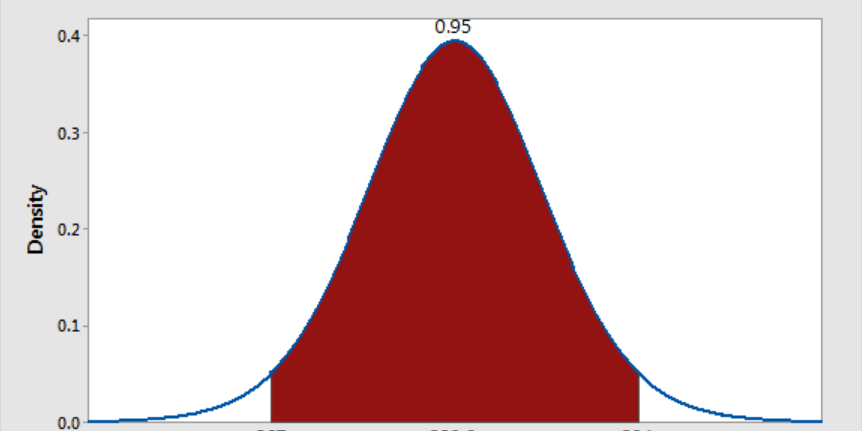
\includegraphics[scale=0.3]{Immagini/intervallo-di-confidenza.png}
		\captionof{figure}{credits: \url{http://blog.minitab.com/blog/adventures-in-statistics-2/understanding-hypothesis-tests\%3A-confidence-intervals-and-confidence-levels}}
	\end{center}
	A questo punto se l'ipotesi nulla è effettivamente vera nel $95\%$ dei casi sarà accettata, mentre solamente nel $5\%$ dei casi sarà rifiutata, cioè per il $95\%$ degli intervalli calcolati per diversi valori osservati sarà accettata, mentre per il rimanente $5\%$ degli intervalli non sarà accettata . Questi intervalli di confidenza sono quelli centrati su valori osservati che sono nella regione del $5\%$ delle code per la distribuzione centrata sull'ipotesi nulla, ovvero quei valori nelle regioni rosse in figura \ref{fig: distro-pvalue}. 
\end{tcolorbox}

\subsection{F measure}
Nel caso sia condotta una regressione con più regressori si può effettuare un test di ipotesi congiunto per i vari parametri che vengono stimati, ovvero vedere se un determinato set di parametri è efficiente o meno nella stima del modello. Quindi è definita la seguente ipotesi nulla:
\begin{equation}
\begin{split}
H_0 &: \; \beta_0 = 0 ,\; \beta_1 = 0,\; \cdot ,\; \beta_k = 0 \\
&:\; \beta_0 =  \beta_1 = \cdot = \beta_k = 0
\end{split}
\end{equation}
che implica l'ipotesi alternativa:
\begin{equation}
H_1: \; \beta_0 \neq 0 ,\; \beta_1 \neq 0,\; \cdot ,\; \beta_k \neq 0
\end{equation}
ovvero si testa se uno tra i parametri stimati sia nullo, se si rifiuta l'ipotesi nulla significa che almeno uno di essi non è nullo, e quindi è significativo.

Il test di ipotesi congiunta si effettua calcolando la F-measure per il modello lineare preso in esame, definita come segue:
\begin{equation}
F = \frac{SSR_r - SSR_{ur}/q}{SSR_{ur}/(n-(k+1))}
\label{F-measure}
\end{equation}
dove $SSR$ rappresenta la somma dei residui al quadrato del modello, cioè la devianza residua. In particolare $SSR_r$ rappresenta la devianza residua per il modello ristretto all'ipotesi nulla, ovvero, supponendo vera l'ipotesi nulla, $SSR_r$ rappresenta la devianza residua del modello in cui i parametri sono posti uguale ai valori specificati dall'ipotesi, in questo caso sono posti uguale a zero. $SSR_{ur}$ rappresenta invece la devianza residua per il modello non ristretto, ovvero quello stimato con tutti i parametri. La variabile $q$ rappresenta invece il numero di restrizioni, ovvero il numero di parametri che sono testati congiuntamente, $n$ rappresenta il numero di osservazioni e $k$ il numero di variabili indipendenti nel modello non ristretto. Le due quantità rapportate nell'equazione \eqref{F-measure} sono distribuite come un $\chi^2$ che implica che la $F$ sia distribuita come una F di Fisher-Snedecor con $q$ e $n-(k+1)$ gradi di libertà. Possiamo quindi impostare un livello di significatività $\alpha$ con il quale rifiutare l'ipotesi nulla. L'ipotesi nulla è accettata se:
\begin{equation}
P(F_0 < F_\alpha) = 1-\alpha
\end{equation}
ovvero se si ottiene un valore per il test $F_0$ minore del valore $F_\alpha$, valore per cui la probabilità è uguale a $1-\alpha$. Questo valore si può trovare tabulato. Se invece si trova un valore maggiore, tale per cui la probabilità di ottenere un valore maggiore o uguale è uguale o minore di $\alpha$, allora si può rigettare l'ipotesi nulla.
\section{Stima dei parametri tramite massima verosimiglianza}
Nel modello lineare classico gli errori si distribuiscono, come si è detto, in modo gaussiano, ovvero:
\begin{equation}
\epsilon_i \sim N(0,\sigma^2)
\end{equation}
così come anche i parametri e le variabili dipendenti, cioè:
\begin{equation}
\begin{split}
b_{OLS} &\sim N(\beta, \sigma^2(X^tX)^{-1}) \\
Y &\sim N(X\beta, \sigma^2 I_n)
\end{split}
\end{equation}
Si può quindi provare a utilizzare stime di massima verosimiglianza che chiedono l'esistenza di n variabili casuali $y_i - X_i\beta$ con $i=1 \cdots n$ che siano identicamente e indipendentemente distribuite condizionatamente al valore $X$ e dipendenti dai parametri $\beta$.\\
Si cerca quindi il valore dei parametri che rendono massima la probabilità di ottenere la verosimiglianza massima:
\begin{equation}
max_\beta L(y_i - X_i\beta) \quad i=1 \cdots n
\end{equation}
Da questo si arriva a dimostrare che lo stimatore dei $\beta$ di massima verosimiglianza (ML) coincide con quello trovato in precedenza, e possiede le stesse proprietà di consistenza, correttezza ed efficienza, comprese le proprietà asintotiche richieste nel caso in cui le misure siano statisticamente indipendenti.

\section{Variabili esplicative qualitative}
Le variabili esplicative qualitative o categoriche sono determinate da attributi:
\begin{itemize}
	\item nominali
	\item ordinali
\end{itemize}
e possono essere:
\begin{enumerate}
	\item dicotomiche (\textit{dummy variables}) se assumono solamente due valori (e.g. sesso);
	\item Politomiche, se assumono più di due valori.
\end{enumerate}

Ora se abbiamo un modello lineare del tipo:
\begin{equation}
Y_i = \beta_0 + \beta_1 D_i + \epsilon_i \quad i=1 \cdots n
\end{equation}
in cui la $D_i$ è una variabili dummy, si ha che essa va ad esercitare il proprio effetto sull'intercetta. Solitamente si riconducono le due possibilità per la variabile dummy ai due valori 0 e 1, per cui quando si ha $D=0$ si ottiene:
\begin{equation}
Y_i = \beta_0 + \epsilon_i
\label{eq: dummy intercetta}
\end{equation}
mentre quando $D=1$, si ottiene:
\begin{equation}
Y_i = \beta_0 + \beta_1 + \epsilon
\label{eq: dummy completa}
\end{equation}
ovvero l'intercetta rappresenta il \textit{valore stimato} di $Y$ quando la variabile esplicativa dummy è uguale a 0. Il coefficiente angolare è dato invece dalla differenza in Y per i due diversi valori della variabile esplicativa dummy, ovvero facendo la differenza tra la \eqref{eq: dummy intercetta} e \eqref{eq: dummy completa}.
La statistica inferenziale si fa anche in questo caso come prima, utilizzando stime e test.

Si può avere anche il caso in cui sia presente sia una variabile qualitativa dummy che una variabile quantitativa. In questo caso si ha un modello del tipo:
\begin{equation}
	y_i = \beta_0 + \beta_1 \cdot x_i + \beta_2 \cdot D_i + \varepsilon_i \qquad \text{con} \quad i=1 \cdots n
	\label{eq: regressione dummy+quantitativa}
\end{equation}
dove la variabile $x_i$ è ovviamente una variabile quantitativa, mentre $D_i$ è la dummy qualitativa che può assumere i due valori $0$ e $1$. In questo caso quindi il parametro $\beta_2$ rappresenta l'effetto della variabile dummy sull'intercetta e osservare quindi se tale effetto risulta significativo oppure no.\\
Il modello per una dummy dicotomica si può quindi scrivere anche come:
\begin{equation}
y_i = 
\begin{cases}
\beta_0 + \beta_1 \cdot x_i + \varepsilon_i \qquad \text{se} \quad D_i = 0 \\
(\beta_0 + \beta_2) + \beta_1 \cdot x_i  + \varepsilon_i \qquad \text{se} \quad D_i = 1
\end{cases}
\end{equation}
da cui si può osservare meglio l'effetto della dummy sull'intercetta del modello.\\
Graficamente questo caso si può visualizzare nel modo seguente:
\begin{figure}
	\centering
	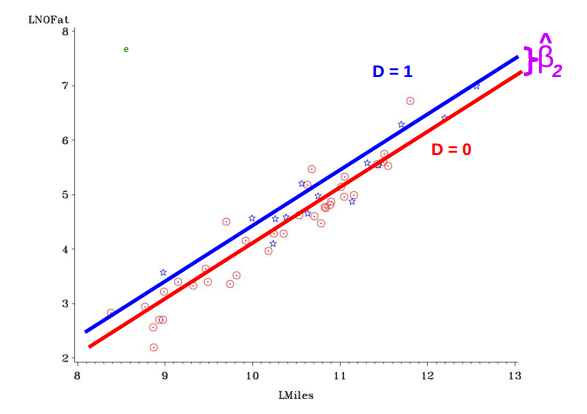
\includegraphics[scale = 0.5]{Immagini/regressione-dummy.png}
	\caption{In figura è riportato un esempio di regressione con dummy variabile dicotomica. In particolare l'esempio rappresenta la regressione $\log(\hat{Y}) = \hat{\beta}_0 + \hat{\beta}_1 \cdot \log(Miles) + \hat{\beta_2} \cdot Seatbelt$, dove $Y$ rappresenta il numero di incidenti fatali, e la variabile dicotomica $D$ è $SeatBelt$.}
\end{figure}